\documentclass[addpoints,a4paper]{exam}

\usepackage{amsmath,amssymb,amsthm}
\usepackage[export]{adjustbox}
\usepackage{graphbox}
\usepackage{graphicx}
\usepackage{hyperref}
\usepackage{makecell}
\usepackage{tabularx}
\usepackage{titling}
\usepackage{listings}
\usepackage{xcolor}

\definecolor{dkgreen}{rgb}{0,0.6,0}
\definecolor{dred}{rgb}{0.545,0,0}
\definecolor{dblue}{rgb}{0,0,0.545}
\definecolor{lgrey}{rgb}{0.9,0.9,0.9}
\definecolor{gray}{rgb}{0.4,0.4,0.4}
\definecolor{darkblue}{rgb}{0.0,0.0,0.6}
\lstdefinelanguage{cpp}{
      backgroundcolor=\color{lgrey},  
      basicstyle=\footnotesize \ttfamily \color{black} \bfseries,   
      breakatwhitespace=false,       
      breaklines=true,               
      captionpos=b,                   
      commentstyle=\color{dkgreen},   
      deletekeywords={...},          
      escapeinside={\%*}{*)},                  
      frame=single,                  
      language=C++,                
      keywordstyle=\color{purple},  
      morekeywords={BRIEFDescriptorConfig,string,TiXmlNode,DetectorDescriptorConfigContainer,istringstream,cerr,exit}, 
      identifierstyle=\color{black},
      stringstyle=\color{blue},      
      numbers=left,                 
      numbersep=5pt,                  
      numberstyle=\tiny\color{black}, 
      rulecolor=\color{black},        
      showspaces=false,               
      showstringspaces=false,        
      showtabs=false,                
      stepnumber=1,                   
      tabsize=5,                     
      title=\lstname,                 
    }

\graphicspath{{images//}}

% Header and footer.
\pagestyle{headandfoot}
\runningheadrule
\runningfootrule
\runningheader{CS 412 Algorithms, Spring 2023}{Homework 2}{\theauthor}
\runningfooter{}{Page \thepage\ of \numpages}{}
\firstpageheader{}{}{}

\boxedpoints

\printanswers

\title{Homework 2\\ CS 412 Algorithms: Design and Analysis}
\author{q1-team-2}  % replace with your team name without the brackets, e.g. q1-team-420
\date{Habib University | Spring 2023}

\begin{document}
\maketitle

\begin{questions}


	\section*{Network Flows}
	\question A group of five persons $P = \{p_1, p_2, ..., p_5\}$ plan to carpool together for each working day $d_i$ of the week. However due to several constraints (such as exams, appointments, etc.), not every person can drive on every day. The following table shows a driving possibility for each person on a given day of the week (i.e. Person $p_i$ can drive on given day $d_i$ if the corresponding element in the table is marked with an `X'):
	
	\begin{table}[h]
		\centering
		\renewcommand{\arraystretch}{1.5}
		\begin{tabular}{llllll}
			      & Mon & Tue & Wed & Thu & Fri \\ \hline
			$p_1$ & X   & X   & X   &     &     \\ \hline
			$p_2$ & X   &     &     &     & X   \\ \hline
			$p_3$ & X   & X   &     & X   &     \\ \hline
			$p_4$ &     & X   &     & X   & X   \\ \hline
			$p_5$ &     & X   &     & X   & X   \\ \hline
		\end{tabular}%
		\caption{Table of Possibilities for each person on a given day of the week} \label{key}
	\end{table}
	
	A schedule is considered to be \textit{feasible} if exactly one person can be assigned one day of the week to drive.
	\begin{parts}
		\part[5] Describe an algorithm using network flows which given the above table of possibilities as an input, computes whether a it is possible to generate a feasible schedule or not? Apply your algorithm to the above table (Table \ref{key}) to determine if it generates a feasible schedule.
		\part[5] What is the time complexity of your algorithm in terms of $n$, where the set of persons $P =  \{p_1, p_2, ..., p_n\}$ and the set of days $D = \{d_1, d_2, ..., d_n\}$
	\end{parts}
	\begin{solution}
		\begin{enumerate}
			\item We can model this problem as a maximum flow problem in a directed graph. We will create a graph \(G=(V,E)\) where \(V\) is set of all nodes and \(E\) is set of all edges. We will create nodes in the graph as follows:
			      \begin{itemize}
				      \item For each person \(p_i\), we create a node \(s_i\), which represents the source of flow for that person.
				      \item For each day \(d_i\), we create a node \(t_i\) which represents the sink of flow for that day.
				      \item For each person-day pair \((p_i,d_j)\), we create a node \(n_{i,j}\) which represents this possibility of person \(p_i\) driving on day \(d_j\).
			      \end{itemize}
			      Now we will add edges to the graph as follows:
			      \begin{itemize}
				      \item For each person \(p_i\), we add an edge \(s_i, n_{i,j}\) for each day \(d_j\) where person \(p_i\) is marked with an \(X\).
				      \item For each day \(d_j\), we add an edge \(n_{i,j}, t_j\) for each person \(p_i\) where person \(p_i\) is marked with an \(X\).
				      \item We add a capacity of 1 to each of the edges \((s_i,n_{i,j})\),\((n_{i,j},t_j)\) and \((p_i,n_{i,j})\).
			      \end{itemize}
			      The intuition behind the graph is that the edge \((s_i,n_{i,j})\) represent the fact that person \(p_i\) can drive on day \(d_j\), the edge \((n_{i,j},t_j)\) represents the fact that day \(d_j\) needs to have one driver, and the edge \((p_i,n_{i,j})\) represent the fact that person \(p_i\) can only drive on day \(d_j\).
			      
			      We can now find the maximum flow in this graph using any standard maximum flow algorithm (such as Ford-Fulkerson). If the maximum flow is equal to the number of days \(|D|\), then we have a feasible schedule. Otherwise, we do not have a feasible schedule.
			      
			      When we apply this algorithm to the above table, we get the following graph:
		\end{enumerate}
	\end{solution}
	
	\section*{Dynamic Programming}
	\question \ \newline
	\begin{minipage}{0.2\linewidth}
		\centering
		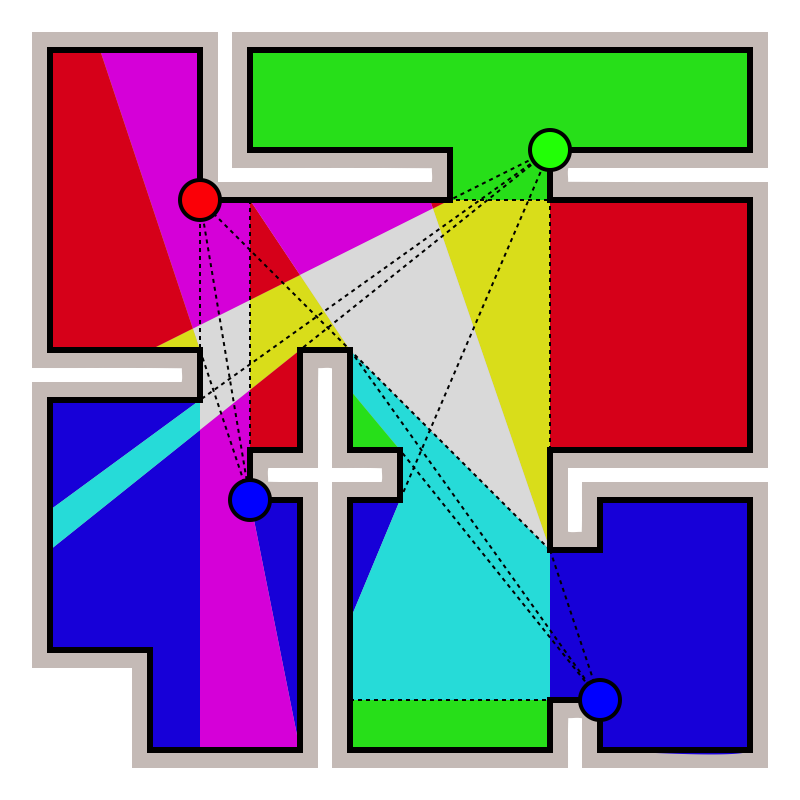
\includegraphics[width=\textwidth,align=t]{gallery}\\
		\href{https://en.wikipedia.org/wiki/Art_gallery_problem}{Wikipedia}
	\end{minipage}
	\hfill
	\begin{minipage}{0.78\linewidth}
		Consider a version of the \href{https://en.wikipedia.org/wiki/Art_gallery_problem}{art gallery problem} where the layout of the gallery is a graph, one or more artworks are placed at each node, and edges represent corridors. Placing a security camera at a node \textit{covers} the artworks at the node and its neighbors.
		\begin{parts}
			\part[5] Design a linear-time dynamic programming approach to find the minimum number of security cameras needed to cover all the artworks.
			\part[5]  Using your approach, determine the nodes at which cameras need to be placed in the gallery whose \href{https://rpruim.github.io/m252/S19/from-class/graphs/graph-representations.html}{edge list representation} is: $\{[n_1,n_2], [n_1, n_3], [n_2,n_4], [n_2, n_5],[n_3,n_6], [n_5, n_7],[n_5,n_8]\}$.
		\end{parts}
	\end{minipage}
	
	\begin{solution}
		\begin{parts}
			\part From the art gallery problem we have that the floor map pf the art gallery can be represented as a simple polygon.
			\\Let $G = (V,E)$ be a graph that represents the map pf the art gallery such that the edges of $G$ represent corridors and the vertices of $G$ represent points where artworks are placed.
			\\\textbf{lemma 1:} If $G$ is a graph contructed from the art gallery where the edges represent the edges and the vertices represent the points where artworks are place, then $G$ will be a tree.
			\\\textbf{Proof:} Let $G = (V,E)$ be a graph constructed from the art gallery such that the edges of $G$ represent corridors and vertices represent points where artworks are placed.
			\\Supppose that $G$ is not a tree, then we have 4 cases,
			\begin{itemize}
				\item \textbf{Case 1:} $G$ is not connected
				      \\If $G$ is not connected then the art galleries floor plan will not be a simple polygon as we have disjoint areas of art gallery with no path between them in the art gallery, so here we have contradiction. So $G$ must be connected.
				\item \textbf{Case 2:} $G$ contains loops.
				      \\If $G$ contains loops then we have a coridor where both ends of the corridor meet at some point, so the floor plan of the art gallery will have a hole in it so the floor plan can't be a simple polygon. Here we have a contradiction, therefore $G$ cannot have loops.
				\item \textbf{Case 3:} $G$ contains multiedges.
				      \\If $G$ contains multiedges then we have a coridor that goes from some point $A$ to some point $B$ and then another corridor that goes from point $B$ to point $A$. If such corrdors exits then the respective floor plan of the art gallery will have a hole.
				      So the floor plan can't be a simple polygon. Here we have a contradiction, therefore $G$ cannot have multiedges.
				\item \textbf{Case 4:} $G$ contains a cycle.
				      \\If $G$ contains a cycle then we have a series of coridors $C_1, C_2, ... C_n$  and a series of points $A_0, A_1, A_2... A_n$ such that every corridor $C_i$ goes from point $A_{i-1}$ to point $A_i$ for $i \in \{1,2,...n-1\}$ and corridor $C_n$ goes from point $A_n$ to point $A_0$.
				      For a art gallery with a floor plan such that such series of corrdors and points exits in it, the floor plan of art gallery will contain a hole.
				      So the floor plan can't be a simple polygon. Here we have a contradiction, therefore $G$ cannot have cyles.
				      
			\end{itemize}
			As we have a contradiction in all 4 cases, the graph $G$ must be a tree.
			\begin{flushright}
				$\square$
			\end{flushright}
			
			% \textbf{lemma 2:} For the graph $G$ contructed from the art gallery where the edges represent the edges and the vertices represent the points where artworks are placed, if $VC$ is a vertex cover of $G$ then if we placing the cameras as each vertex $v \in VC$ is necessary and sufficient to cover all artworks,
			% and if $VC$ is the minimum vertex cover then $|VC|$ is the minimum number of cameras required to cover all artworks.
			% \\\textbf{Proof:} 
			% Let $G =(V,E)$ be a graph contructed from the art gallery where the edges represent the edges and the vertices represent the points where artworks are placed. Let $VC$ be a vertex cover of $G$.
			% \\First we show that placing cameras on each $v \in VC$ is sufficient to cover all the artworks.
			% \\Suppose we place a camera at each vertex $v \in VC$, we know that each $v \in VC$ is covered as cameras are placed at them.
			% \\Now are $VC$ is the vertex cover of $G$ then for each edges $e \in E$ where $e = \{u,v\}$ such that $e$ connects vertex $u$ to vertex $v$, we have that $v \in VC$ or $u \in VC$.
			% \\Without loss of generality suppose $v \in VC$ then we have that $v$ is covered, and as $u$ is a neighbor of $v$ then by placing a camera on $v$ covers $u$ as well. As $G$ is a tree (from lemma 1) we have that $G$ is connected, therefore $\forall v \in V$, $v$ has an edge connected to it, so placing a camera on each vertex $v \in VC$ covers all the artworks.
			% \\\\Next we show that placing cameras on each $v \in VC$ is necessary to cover all the artworks.
			% \\Let $C$ denote the set of vertices of $G$ where the cameras are placed such that all the artworks are covered.
			% We have that for each vertex $v \in V$ we have that $v \in C$ or we have a vertex $u$ neighbor of $v$ such that $u \in C$. 
			% Suppose $C$ is not a vertex cover of $G$ then we have an edge $e = \{u,v\} \in E$ such that $u \not\in C$ and $v \not\in C$.
			% Now if both $u$ and $v$ are not in $C$ then we have vertices $u'$ neighbor of $u$ and $v'$ neighbor of $v$ such that $u' \in C$ and $v' \in C$.
			
			% \\As $G$ is a tree there are no cycles in $G$, then for each edges $e = \{u,v\} \in E$ we have that either 
			Now we will devise a linear time dynamic programming approach to solve this problem by taking the following steps:
			\begin{enumerate}
				\item Characterize the structure of an optimal solution.
				\item Recursively define the value of an optimal solution.
				\item Show how the value of an optimal solution can be computed in a bottom-up manner.
				\item Argue about the time complexities of our approach.
			\end{enumerate}
			\textbf{Characterize the structure of an optimal solution.}
			\\Let $P$ be a simple polygon that represents the floors map of an art gallery, let $G = (V,E)$ be a graph constructed from $P$ such that the edges of $G$ represents corridors and the vertices of $G$ represents points where artworks are places.
			Then for out problem the value of an optimal solution would be a set of verties $C \subseteq V$ such that placing cameras at vertices $v \in C$ covers the entire art gallery and if there exits a set of vertices $Z \subseteq V$ such that placing cameras 
			at vertices $v \in Z$ covers the entire art gallery then $|C| \leq |Z|$.
			\\The value of the optimal solution would be the integer $n = |C|$.
			\\\\\textbf{Recursively define the value of an optimal solution.}
			\\Let $P$ be a simple polygon that represents the floors map of an art gallery, let $G = (V,E)$ be a graph constructed from $P$ such that the edges of $G$ represents corridors and the vertices of $G$ represents points where artworks are places.
			From lemma 1 we know that $G$ is a tree. We pick $r \in V$ to be the root of the tree $G$.
			\\Let $H(v)$ denote the set of all children of vertex $v \in V$, and let $R(v)$ denote the set of all grandchildren of vertex $v \in V$.
			\\The value of the optimal solution for a subtree $T \subset G$ rooted at vertex $x$ can be computed as follows (we denote the value of the optimal solution as $f(x)$):
			$$f(x) = \text{min}\left(\left\{1 + \sum_{v \in H(x)}f(v), |H(x)| + \sum_{v \in R(x)}f(v)\right\}\right)$$
			This is because at every subtree $T \subset G$ rooted at vertex $x$, we have 2 options, either $x$ is in the optimal solution (we place a camera on $x$) or $x$ is not in the optimal solution (we don't place a camera on $x$). 
			If we don't place a camera on $x$ then we must place a camera on all the neighbors of $x$ therefore all the childern of $x$ must be in the optimal solution.
			If we place a camera on $x$ then we have recursively compute the optimal solution for all the subtrees rooted at a childern of $x$ and add 1 to it. The optimal solution would be the minimum of the 2 options.
			\\\\\textbf{Show how the value of an optimal solution can be computed in a bottom-up manner.}
			The value of the optimal solution can be computed in a bottom-up manner as follows:
			\\Let $P$ be a simple polygon that represents the floors map of an art gallery, let $G = (V,E)$ be a graph constructed from $P$ such that the edges of $G$ represents corridors and the vertices of $G$ represents points where artworks are places. 
			Let $r$ be the root vertex of $G$.
			\\We define function $F(G)$ that computes the value of the optimal solution in a bottom-up manner.
			% \begin{lstlisting}
			
			% \end{lstlisting}
			$F(G):$
			\begin{enumerate}
				\item Label each vertex $v \in V$ with an integer $i \in \{1,2,...|V|\}$
				\item Construct a $|V| \times 2$ array $A$, where each $A[i][0]$ represent the value of a solution by placing a camera at $i^{\text{th}}$ vertex, and each $A[i][1]$ represent the value of a solution by not placing a camera at $i^{\text{th}}$ vertex.
				\item Let $L_n$ be the set of all vertices at level $n$. For each level $i$ of $G$, $\forall x \in L_i$ compute $A[x][0]$ and $A[x][1]$. If $x$ is a leaf vertex then $A[x][0] = 1$ and $A[x][1] = 0$, else compute $A[x][0]$ and $A[x][1]$ by using the following recurence
				      $$f(x) = \text{min}\left(\left\{1 + \sum_{v \in H(x)}f(v), |H(x)| + \sum_{v \in R(x)}f(v)\right\}\right)$$ we compute $f(v)$ for $v \in R(x)$ or $f(v)$ for $v \in H(x)$ each time by looking the values of $A[v][0]$ and $A[v][1]$.
				\item Return min$(\{A[r][0],A[r][1]\})$
			\end{enumerate}
			This we start from the bottom level and move up to the top level and compute the value of the optimal solution in a bottom up manner.
			\\\\\textbf{Argue about the time our approach.}
			\\The algorithm start from the bottom level and move to the top level visiting each vertex and computing the value of the solution for the tree rooted at that vertex. The values of the solutions of subproblems are stored in an array and looked up from ther each time.
			Step 1 and 2 takes $O(|V|)$ time, then we go to each vertex once and only look up the values of its childern, the total number of childern to look up are equal to $|E|$ as each child vertex has 1 edges ascosiated to it (children and child vertex are just non-root vertex). so step 3 takes $O(|V| + |E|)$ time.
			Step 4 takes $O(1)$ time.
			\\So our algorithm takes $O(|V|) + O(|V|) + O(|V|+|E|) + O(1) \in O(|V|+|E|)$ time, therefore our algorithm is linear time
			% at max a vertex has $\Delta(G)$ childern where $\Delta(G)$ is the maximum degree of $G$, so step 3 takes $O(|V|)$ 			
			\part We place cameras at vertices $n_2$, $n3$, $n_7$, and $n_8$, giving the value of the optimal solution as $4$.
			$\{n_1,n_4,n_5,n_6\}$ is also a valid placement of cameras with the same value.
		\end{parts}
		
	\end{solution}
	
	\question \ \newline
	\begin{minipage}[m]{0.25\linewidth}
		\centering
		\ \newline
		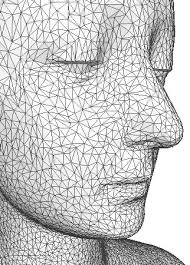
\includegraphics[width=.8\textwidth,valign=t]{mesh}\\
		\href{http://glasnost.itcarlow.ie/~powerk/GeneralGraphicsNotes/meshes/polygon_meshes_old.html}{\small 3D Object Representations}
	\end{minipage}
	\hfill
	\begin{minipage}[t]{0.73\linewidth}
		\begin{tabularx}{\textwidth}{Xc}
			Modern rendering hardware is optimized for triangles. Any 3D object to be rendered has to be \textit{triangulated}, because of which the \textit{triangle mesh} is the de-facto choice of representation for 3D objects. It is known that any polygon can be triangulated, however the triangulations are not generally unique.
			 & 
			\makecell[t]{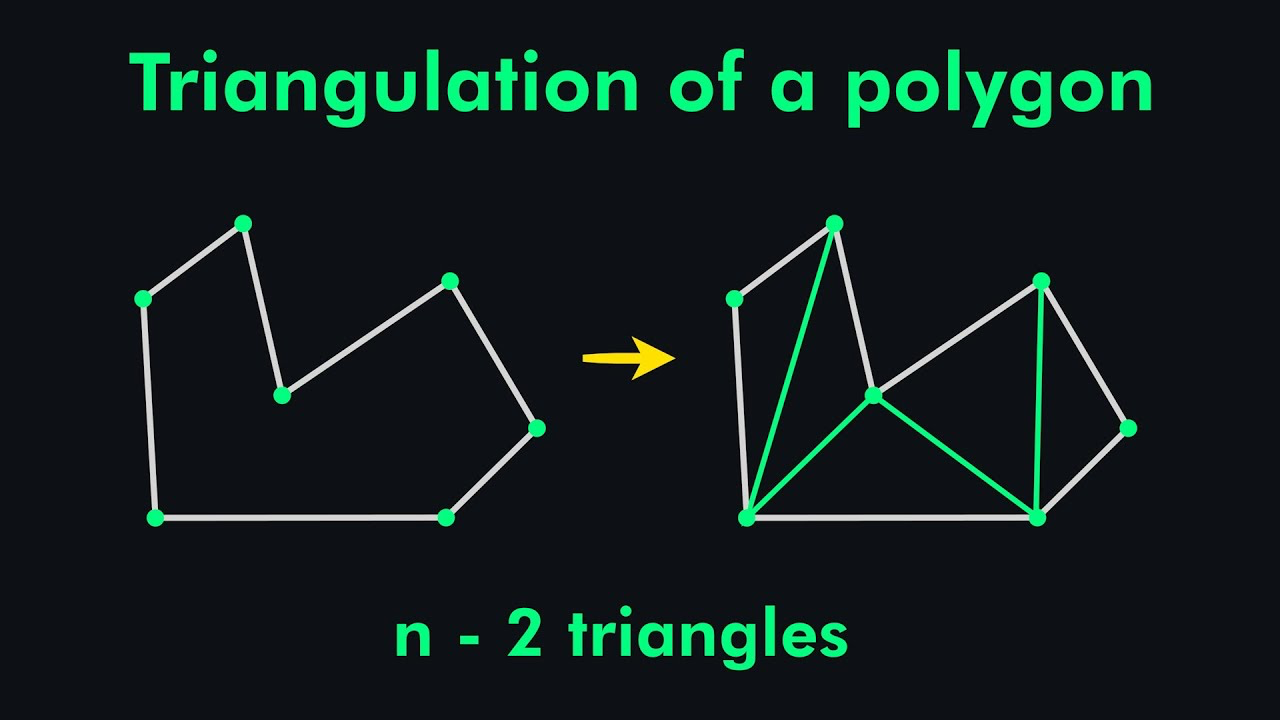
\includegraphics[width=.35\textwidth,valign=t]{triangulate} \\
				\href{https://www.youtube.com/watch?v=2x4ioToqe_c}{YouTube}}
		\end{tabularx}
		\begin{parts}
			\part[5] Devise a dynamic programming approach to compute the number of triangulations of a polygon with $n$ vertices.
			\part[5] Argue about the complexity of your approach.
		\end{parts}
	\end{minipage}
	
	\begin{solution}
		\begin{parts}
			\part We use dynamic programming to devise an approach to compute the number of triangulations of an n-gon.
			From theorem 1.19 from the following text \href{http://assets.press.princeton.edu/chapters/s9489.pdf}{http://assets.press.princeton.edu/chapters/s9489.pdf}
			we have that for a \textit{convex} n+2-gon the number of triangulations are given by the $n^{\text{th}}$ catalan number $C_n = \frac{1}{n+1} {2n \choose n}$.
			\\However we do not have a closed form to compute the number of trangulations of concave polygon however we do have a bound that is for a n+2-gon the number of triangulations are between 1 and $C_n$ (Theorem 1.20 from \href{http://assets.press.princeton.edu/chapters/s9489.pdf}{http://assets.press.princeton.edu/chapters/s9489.pdf}).
			\\We devise a dynamic programming approach to compute the number of different triangulations by doing the follwong steps.
			\begin{enumerate}
				\item Characterize the structure of the solution.
				\item Recursively define the value of the solution.
				\item Show how the value of the solution can be computed in a bottom-up manner.
			\end{enumerate}
			\textbf{Characterize the structure of an optimal solution.}
			\\Let $P$ be a polygon with $n$ vertices. The solution will be a set $T = \{p_1,p_2,...p_m\}$ where each $p_i$ is some triangulation of $P$, and $T$ contains all possible triangulations of $P$.
			\\The value of the solution would be the integer $k = |T|$.
			\\\textbf{Recursively define the value of the solution.}
			\\Our approach to compute the value of the solution would be the following:
			\\We will draw all possible diagonals of $P$, each time we draw a diagonal in $P$ we obtain 2 polygons $P_1$ and $P_2$. 
			We recursively compute the number of triangulations of polygon $P_1$ and $P_2$. Our base case would be a triangle, where number of traingulations are $1$ as in drawing no daigonals.
			We sum the number of traingulations after drawing each daigonal in $P$ and that would be the number of different traingulations of $P$.
			\\The video provides an algorithm to draw a valid daigonal in $P$ \href{https://www.youtube.com/watch?v=2x4ioToqe_c}{YouTube}. 
			\\We represent each daigonal with a set of vertices $\{u,v\}$ where daigonal has end points $u$ and $v$. We define function $F(P)$ that computes the value of the solution as follows:
			\\$F(P):$
				\begin{enumerate}
					\item If $P$ is a triangle return 1
					\item Let tringulations = 0, let daig = $\emptyset$
					\item Else, for each vertex $v$ of $P$,
					      \begin{itemize}
						      \item If $v$ is convex then for each other vertex $u$ of $P$
						      \item if there exists a daigonal $\{v,u\}$ then draw the daigonal $D$
						      \item If $D\not\in$ daig, then daig = daig $\cup$ $\{D\}$, and obtain polygons $P_1$ and $P_2$
						      \item tringulations = tringulations + $F(P_1) \times F(P_2)$
					      \end{itemize}
					\item Return triangulations
				\end{enumerate}
				\textbf{Show how the value of the solution can be computed in a bottom-up manner.}
				\\The value of the solution can be computed in a bottom-up manner as follows,
				\\$F(P):$
			\begin{enumerate}
				\item Label the vertices of $P$ with integers from 1 to $n$
				\item Construct a $n\times n$ array $A$ where each entry $A[i][j]$ represents the number of triangulations of the polygon obtained by drawing a daigonal from vertex $i$ to vertex $j$,
				      As we obtain 2 polygons from this daigonal we store the num,ber of triangulations of 1 in $A[i][j]$ and other in $A[j][i]$.
				\item For each $i \in \{1,2,..n\}$ and for each $j \in \{1,2,..n\}$
				      \begin{itemize}
					      \item Check if theres a valid daigonal from $i$ to $j$
					      \item if there exists a daigonal $\{i,j\}$ then draw the daigonal $D = \{i,j\}$
					      \item If $D\not\in$ daig, then daig = daig $\cup$ $\{D\}$, and obtain polygons $P_1$ and $P_2$
					      \item tringulations = tringulations + $F(P_1)\times F(P_2)$
				      \end{itemize}
				\item If $P$ is a triangle return 1
				\item Let tringulations = 0, let daig = $\emptyset$
				\item Else, for each vertex $v$ of $P$,
				      
				\item Return triangulations
			\end{enumerate}
			
			\part
		\end{parts}
		
	\end{solution}
	
	\section*{Greedy Algorithms}
	
	\question
	The \textit{coin change} problem is as follows.
	
	\begin{quote}

		\underline{Input}:
		\begin{itemize}
			\item A non-empty set of positive coin denominations $d_1, d_2, \ldots, d_n$.
			\item A positive integer $m$.
		\end{itemize}
		\underline{Output}: The minimum number of coins required to make change for $m$.
	\end{quote}
	Mathematically, we want to minimize the total number of coins $\sum c_i$ such that $\sum c_i d_i = m$.
	\begin{parts}
		\part[5] Given coin denominations, $1,2,4,8,\ldots,2^k$, and a positive amount, $m<2^{k+1}$, provide an $O(\lg m)$-time algorithm to find the minimum number of coins required to make change for $m$. Justify the correctness and complexity of your algorithm.
		\part[5] Provide a set of denominations for which you can prove that the greedy approach correctly finds the minimum number of coins required to make change. Also provide the proof.
		\part[5] Compare and contrast this problem with the knapsack problem.
	\end{parts}
	
	\begin{solution}
		\begin{enumerate}
			\item We know that for a number \(m\) represented in \(r\) base has \(\lfloor\log_{r}(m)\rfloor\) digits. So, the representation of the number in base \(r\) would mean,
			      \[m=\sum_{i=0}^{\lfloor\log_{r}(m)\rfloor}a_ir^i\]
			      Where, \(a_i\) is the digit at the \(i^{th}\) place. The coin change problem is about finding the minimum number of coins required to make change for \(m\), and the denomination is powers of \(2\). So, the mathematical representation of the coin change problem would be,
			      \[m=\sum_{i=0}^{k}d_i2^i\]
			      Where, \(a_i\) is the digit at the \(i^{th}\) place. So, the minimum number of coins required to make change for \(m\) would be the number of digits in the representation of \(m\) in base \(2\). This is very similar to the representation of the number in base \(r\). Infact it is the exact same thing. As we have established above that the number of digits in the representation of \(m\) in base \(r\) is \(\lfloor\log_{r}(m)\rfloor\). So, the minimum number of coins required to make change for \(m\) would be less than or equals to \(\lfloor\log_{2}(m)\rfloor\). We have implemented this algorithm in C++ below.
			      \begin{lstlisting}[language=cpp]
#include <cassert>
#include <iostream>

const uint32_t coinChange(uint32_t n) {
	uint32_t sum = 0u;
	while (n) {
		sum += n & 0x1;
		n >>= 1;
	}
	return sum;
}

int main(void) {
	assert(coinChange(0u) == 0u);
	assert(coinChange(1u) == 1u);
	assert(coinChange(2u) == 1u);
	assert(coinChange(3u) == 2u);
	assert(coinChange(4u) == 1u);
	assert(coinChange(5u) == 2u);
	assert(coinChange(6u) == 2u);
	assert(coinChange(7u) == 3u);
	assert(coinChange(8u) == 1u);

	std::cout << "All tests passed!" << std::endl;

	return 0;
}
			\end{lstlisting}
			      \begin{lstlisting}[language=cpp]
$ g++ -std=c++11 -o coinChange coinChange.cpp
$ ./coinChange
				\end{lstlisting}
			      The complexity of this algorithm is \(O(\lg m)\) because we are only using the digits of the number \(m\) in base \(2\) to make change for it. We are not using any other information about the number \(m\).
			      
			\item For a positive integer \(m\), we can take a denomination to be \(\{n|n\in\mathbb{N}\land n<m\}\). We can prove the correctness of the algorithm because there are only two coins required from these denominations to make change for any positive integer \(m>1\) that are \(\{1, m-1\}\) and for \(m=1\) we need one coin that is \(\{1\}\). The complexity of this algorithm is \(O(1)\) because we are only using two coins to make change for any positive integer \(m>1\).
			\item The coin change problem is similar to knapsack problem, the difference between the two is that in the coin change problem we are given a set of denominations and we have to find the minimum number of coins required to make change for \(m\) using these denominations. In the knapsack problem we are given a set of items and we have to gather the items that would give us the maximum value without exceeding the capacity of the knapsack.
		\end{enumerate}
		
		
	\end{solution}
	
\end{questions}

\end{document}

%%% Local Variables:
%%% mode: latex
%%% TeX-master: t
%%% End:
